In class, we talked about how we need to do training/test split to make sure that our model is generalizing well. We also discussed how we should not reuse a test set too much, because otherwise the test accuracy may not be an accurate measure of the accuracy on the data distribution. In reality, a ML model often has many \emph{hyper-parameters} which need to be tuned (we will see an example in this question). We don't want to use the test set over and over to see what the best value of this hyper-parameter is. The solution is to have a third split of the data, and create a \emph{validation set}. The idea is to use the validation set to evaluate results from the training set and tune any hyper-parameters. Then, use the test set to double-check your evaluation after the model has ``passed" the validation set. Please see this nice explanation for more discussion: \url{https://developers.google.com/machine-learning/crash-course/validation/another-partition}.

With this final piece, we are now ready to build a real ML pipeline. It usually conducts three parts. (1) Load and pre-process the data. (2) Train a model on the training set and use the {validation set} to tune hyper-parameters. (3) Evaluate the final model on the test set and report the result.

In this problem, you will implement the \emph{$k$-nearest neighbor ($k$-NN) algorithm} to conduct classification tasks. We are providing starter bootstrap code and you are expected to complete the classes and functions. The dataset we will use is a subset of Breast Cancer Wisconsin (Diagnostic). This is a binary classification dataset. Each data point is represented by $(x_i, y_i)$ with $x_i\in \R^{30}$ and $y_i\in \{0,1\}$. A sample data point is $(x_i,y_i)$ is $$x_i=[19.17, 24.8, \dots , 0.1767, 0.3176, 0.1023], \; y_i=0.$$ More explanations are available on \url{https://archive.ics.uci.edu/dataset/17/breast+cancer+wisconsin+diagnostic}.

\subsubsection*{$k$-NN algorithm}
The $k$-nearest neighbor ($k$-NN) algorithm is one of the simplest machine learning algorithms in the supervised learning paradigm. The idea behind $k$-NN is simple, and we explain it first for the case of $k=1$. The 1-NN algorithm predicts the label of any new datapoint $\x$ by finding its closest neighbor $\x'$ in the training set, and then predicts the label of $\x$ to be the same as the label of $\x'$. For general $k$, the $k$-NN algorithm predicts the label by taking a majority vote on the $k$ nearest neighbors.

%$k$-NN algorithm assumes the similarity between the new case (testing instance) and available cases (training data) and assigns the new case's category based on the top-k most similar available cases.

We now describe the algorithm more rigorously. Given a hyper-parameter $k$, training instances $(\mathbf{x}_i, y_i)$ ($\mathbf{x}_i \in \mathbb{R}^d$ and $y_i$ is the label), and a test example $\mathbf{x}$, the $k$-NN algorithm can be executed based on the following steps, 
\begin{enumerate}[topsep=5pt, itemsep=-2pt]
    \item Calculate the \emph{distances} between the test example and each of the training examples.
    \item Take the $k$ nearest neighbors based on the distances calculated in the previous step.
    \item Among these $k$ nearest neighbors, count the number of the data points in each class.
    \item Predict the label $\hat{y}$ of $\x$ to be the most frequent class among these neighbors (we describe how to break any ties later). 
    %Assign prediction $y$ as the category for which the number of the neighbors is maximum.
\end{enumerate}

You are asked to implement the missing functions in \colorbox{Gainsboro!60!Lavender}{knn.py} following each of the steps.

\subsubsection*{Part 3.1 Report 4-nearest neighbor accuracy (\blue{8pts})}
\paragraph{Euclidean distance calculation}
Compute the distance between the  data points based on the following equation:
\begin{equation}
    d(\mathbf{x}, \mathbf{x}') = \|\mathbf{x}-\mathbf{x}'\|_2 = \sqrt{\sum_{i=1}^{d}(x_i-x'_i)^2}.
\end{equation}

\noindent \emph{Task}: Fill in the code for the function \colorbox{Gainsboro!60!Lavender}{compute\_l2\_distances}.

\paragraph{$k$-NN classifier}
Implement a $k$-NN classifier based on the above steps. Your algorithm should output the predictions for the test set.
\emph{Note:} You do not need to worry about ties in the distance when finding the $k$ nearest neighbor set. If this is a tie in the majority label of the $k$ nearest neighbor set, just return 0 as the label.\\

\noindent \emph{Task}: Fill in the code for the function \colorbox{Gainsboro!60!Lavender}{predict\_labels}.

\paragraph{Report the error rate}
We want you to report the error rate for the classification task. The error rate is defined as:
\begin{equation}
    \text{error rate} = \dfrac{\text{\# of wrongly classified examples}}{\text{\# of total examples}}.
\end{equation}

\noindent \emph{Task}: Fill in the code for the function \colorbox{Gainsboro!60!Lavender}{compute\_error\_rate}.\\

\noindent \textbf{Report Item}: Report the error rate of your $k$ nearest neighbor algorithm in the validation set when $k=4$ using Euclidean distance.\\

\textit{Comment:} The validation error rate is 0.07692307692307693 (7.69\%) when k = 4 using Euclidean distance.

\subsubsection*{Part 3.2 Data transformation (\blue{2+2pts})}
We are going to add one more step (data transformation) in the \colorbox{Gainsboro!60!Lavender}{data\_processing} part and see how it works. Data transformations and other feature engineering steps often play a crucial role to make a machine learning model work.  Here, we take two different data transformation approaches. This link might be helpful: \url{https://en.wikipedia.org/wiki/Feature_scaling}.

\paragraph{Normalizing the feature vector}
This one is simple but sometimes may work well. Given a feature vector $\mathbf{x}$, the normalized feature vector is given by $\mathbf{\tilde{x}}=\dfrac{\mathbf{x}}{\|\mathbf{x}\|_2}$. If a vector is an all-zero vector, define the normalized vector to also be the all-zero vector (in practice, a useful trick is to add a very very small value to the norm of $\mathbf{x}$, so that we do not need to worry about  division by zero).

\paragraph{Min-max scaling for each feature}
The above normalization is independent of the rest of the data. On the other hand, min-max normalization scales each sample in a way that depends on the rest of the data. More specifically, for each feature in the training set, we normalize it linearly so that its value is between 0 and 1 across all samples, and in addition, the largest value becomes exactly 1 while the smallest becomes exactly 0. Then, we will apply the same scaling parameters we get from training data to our test instances.\\

\noindent \emph{Task}: Fill in the code for the function \colorbox{Gainsboro!60!Lavender}{data\_processing\_with\_transformation}.\\

\noindent \textbf{Report Item}: Report the error rate of your $k$ nearest neighbor algorithm in the validation set for $k=4$ using Euclidean distance when data is using (1) Normalized featured vector, and (2) Min-max scaling featured vector.\\

\textit{Comment:}
\begin{itemize}
  \item The validation error rate is 0.0440 (4.40\%) in Problem Set 1.2 when using normalization.
  \item The validation error rate is 0.0549 (5.49\%) in Problem Set 1.2 when using minmax\_scaling.
\end{itemize}

\subsubsection*{Part 3.3 Different distance measurement (\blue{3pts})}

In this part, we will change the way that we measure distances. We will work with the original (unnormalized) data for simplicity, and continue the experiments from Part 3.1. 
% \paragraph{Minkowski distance calculation}
% Compute the distance between data points based on the following equation:
% \begin{equation}
%     d(\mathbf{x}, \mathbf{x}') = \|\mathbf{x}-\mathbf{x}'\|_3 = \sqrt[3]{\sum_{i=1}^{n}|x_i-x'_i|^3}
% \end{equation}

% \noindent \emph{Task}: Fill in the code for the function \colorbox{Gainsboro!60!Lavender}{compute\_minkowski\_distance} and change distance function used in the main function in the code to get results.

\paragraph{Cosine distance calculation}
Compute the distance between data points based on the following equation:
$$ d(\mathbf{x}, \mathbf{x}')=\left\{
\begin{array}{lcl}
1, &  & \text{if } \|\mathbf{x}\|_2 = 0 \text{ or } \|\mathbf{x}'\|_2 = 0 \\
1- \dfrac{\mathbf{x} \cdot \mathbf{x}'}{\|\mathbf{x}\|_2\|\mathbf{x}'\|_2} & & \text{otherwise}.
\end{array}
\right.
$$

Similar to when we are normalizing the feature vector, a useful trick in practice is to add a  very small value to the norm of $\mathbf{x}$, so that we do not need to worry about  division by zero issues.\\

\noindent \emph{Task}: Fill in the code for the function \colorbox{Gainsboro!60!Lavender}{compute\_cosine\_distances} and change distance function used in the main function in the code to get results.\\

\noindent \textbf{Report Item}:  Report the error rate of your $k$ nearest neighbor algorithm in the validation set for $k=4$ using cosine distance for \emph{original data without data transformation}.\\

\textit{Comment:}
\begin{itemize}
\item The validation error rate is 0.0440 (4.40\%) in Problem Set 1.3, which use cosine distance
\end{itemize}

\subsubsection*{Part 3.4 Tuning the hyper-parameter $k$ (\blue{10pts})}
Again, follow Part 3.1, however, this time we conduct experiments with $k=\{1, 2, 4, 6, 8, 10, 12, 14, 16, 18\}$ on the original dataset without data transformation.\\

\noindent \emph{Task}: Fill in the code for the function \colorbox{Gainsboro!60!Lavender}{find\_best\_k}. Recall that the choice of best hyperparameter is based on validation set.\\

\noindent \textbf{Report Item}: (1) Report and draw a curve based on the error rate of your model on the \emph {training set} for each $k$. What do you observe? (\blue{2pts}) (2) Report and draw a curve based on the error rate of your model on the \emph {validation set} for each $k$. What is your best $k$? (\blue{2pts}) (3) What do you observe by comparing the difference between the two curves? (\blue{2pts}) (4) What is the final test set error rate you get using your best-$k$? (\blue{1pt}) (5) Comment on these results from the perspective of overfitting, generalization and hyper-parameter tuning. (\blue{3pts}).\\

\textit{Comment:}
\begin{enumerate}
  \item The training error rate generally increases as $k$ increases, since the KNN classifier becomes less flexible and the decision boundary becomes smoother.
  
  \begin{figure}[H]
    \centering
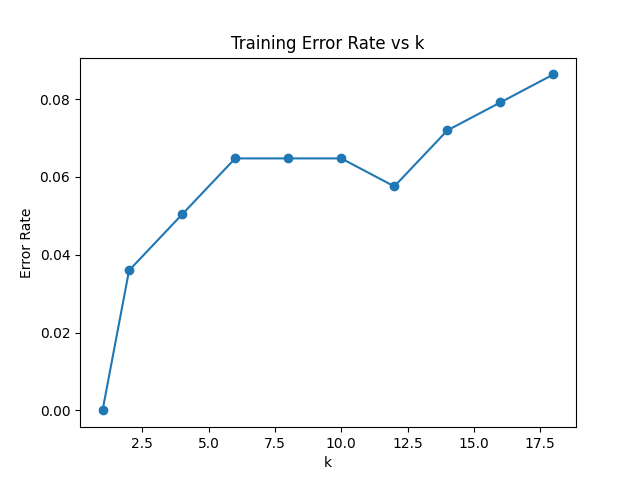
\includegraphics[width=0.6\linewidth]{Train_Error_vs_k.png}

    \caption{Training error rate as a function of $k$.}
    \label{fig:train_error}
  \end{figure}

  \item Based on the validation set, the best choice of $k$ is $6$.
  
  \begin{figure}[H]
    \centering
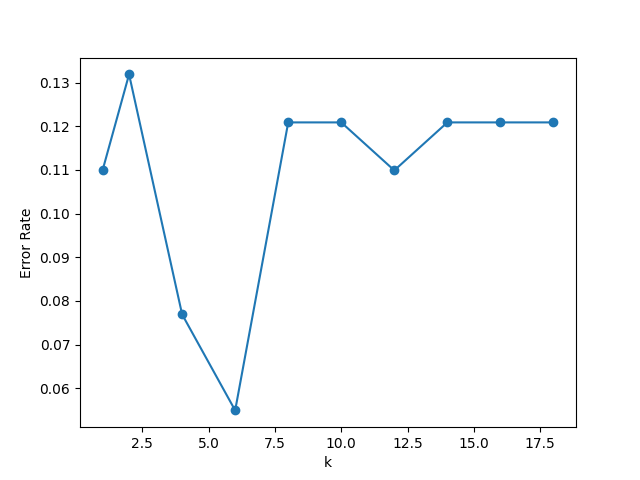
\includegraphics[width=0.6\linewidth]{Val_Error_vs_k.png}

    \caption{Validation error rate as a function of $k$.}
    \label{fig:val_error}
  \end{figure}

  \item On the training set, the error rate monotonically increases with larger $k$. On the validation set, the error rate first decreases and then increases as $k$ increases.

  \item Using the best $k=6$, the final test error rate is $0.0710$ (7.10\%).

  \item For small $k$, the model tends to overfit the training data and generalizes poorly. For large $k$, the model underfits due to excessive smoothing. The validation set is used for hyper-parameter tuning because it provides a less biased estimate of generalization performance than the training set. Selecting $k$ based on the minimum validation error achieves a good balance between overfitting and underfitting.
\end{enumerate}

\iffalse
\subsubsection*{Part 3.5  (\blue{0pts})}

\noindent \textbf{Report Item}: Include your filled-in code in the submitted pdf file.
\fi

\subsubsection*{Code submission}

Make sure to include your complete filled-in code in the single zip file that you upload for all your codes for the HW.